%Technology: precise description of the technology / approach that is used

% Inspiré de la section 10 du papier formose

\begin{figure}[t]
    \centering
    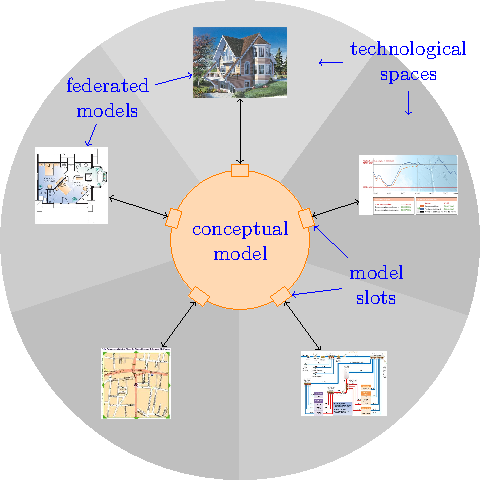
\includegraphics[width=\columnwidth]{Figures/federation.pdf}
    \caption{The model federation approach}
    \label{fig:mf}
\end{figure}

To meet the \mlpc, we have decided to use the general
approach of model federation~\parencite{Golra2016-federation}. \emph{Model
  federation} is a way to assemble models using some kind of
low-coupling links. It has been studied to answer the \OMG' RFP
Semantic Modeling for Information Federation~\parencite{simf}. In
contrast to approaches that compose metamodels into a single large
metamodel grouping all needed entities, model federation build links
between models and metamodels (even through levels) to make ``things''
work together. As an illustration of this feature, we developed a
free-modeling editor -- freeing oneself from the bonds of
model/metamodel conformity -- that is presented
in~\parencite{models2016-freemodel}. Another notable feature of
this approach is the strong decoupling among tools that remain usable
after federations are made.

We decided to use this approach since it offers the possibility to
link and to navigate among levels. Before we describe the overall
architecture in next section, here are some key concepts implemented
in the Openflexo~\parencite{openflexo_link} framework.

% figure
% Dans la suite les références à la figure sont commentés


\begin{figure*}
    \centering
    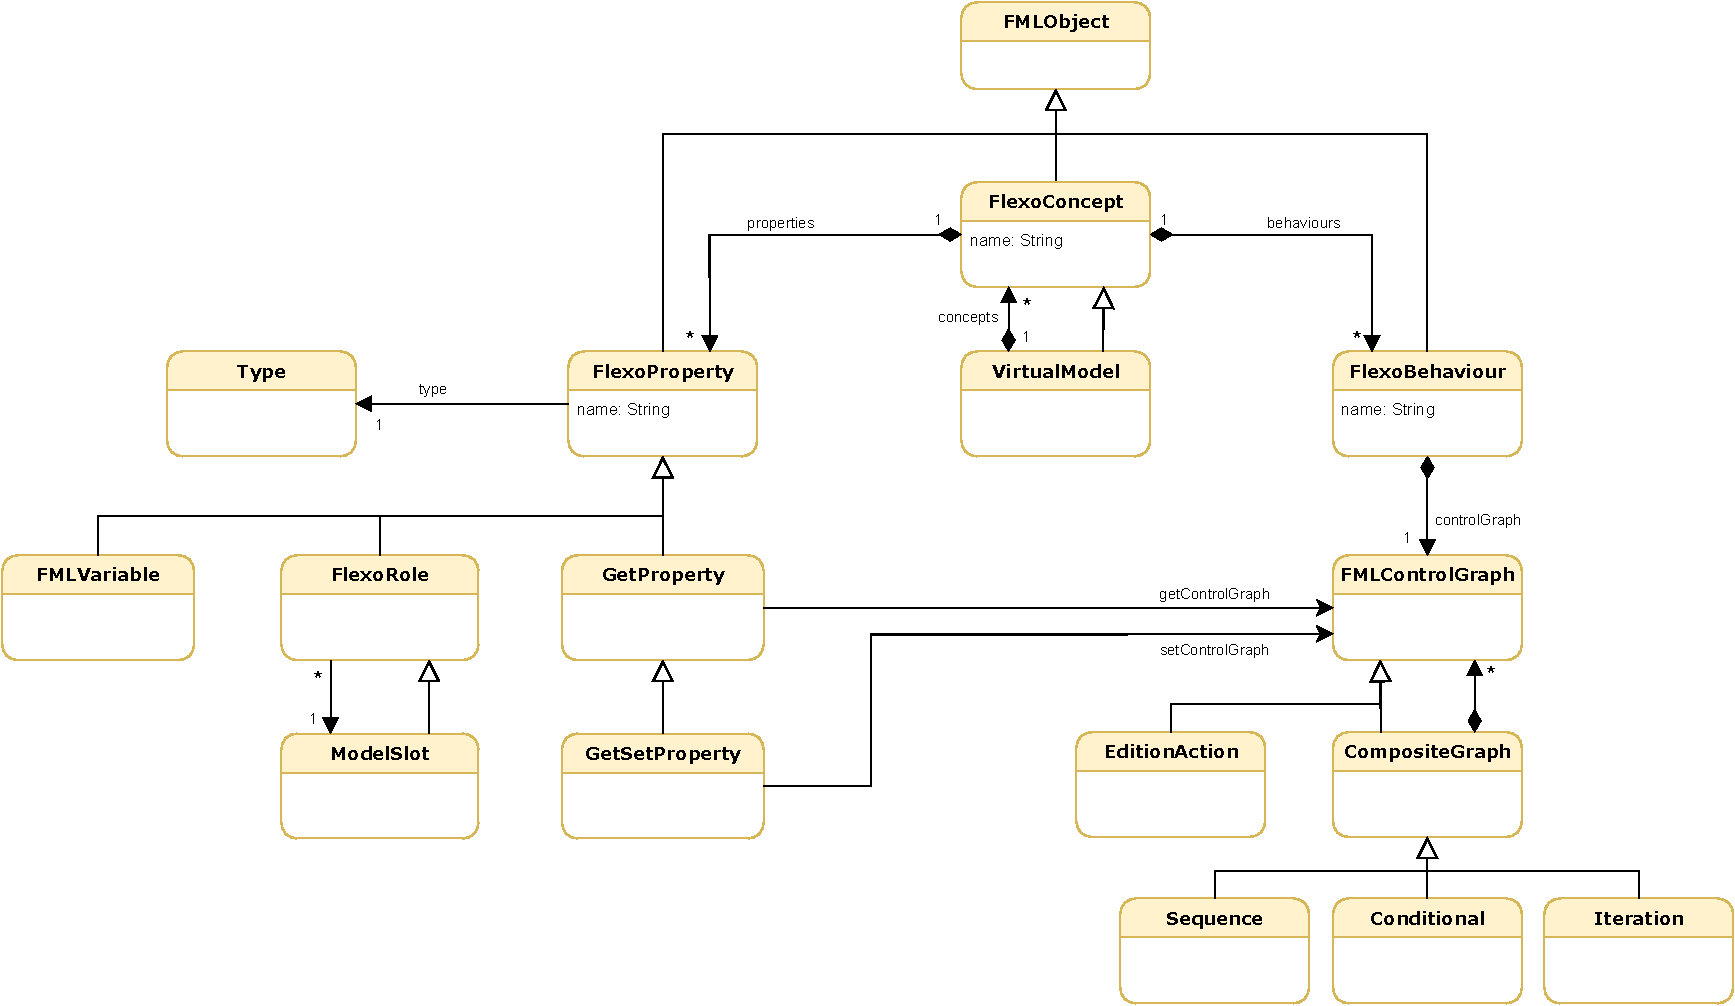
\includegraphics[width=1.0 \textwidth]{Figures/FMLMetaModel.pdf}
    \caption{Representation of the main concepts of \FML language}
    \label{fig:mm}
\end{figure*}
%\noteAntoine{Dans la figure ne manque-t-il pas les containements ? (VM vers Concepts)}
%\noteSylvain{C'est le cas dans cette nouvelle figure}

This framework relies on the architecture of Figure~\ref{fig:mf}. A federation
gathers a set of conceptual models, named \emph{virtual models} and a
set of \emph{federated models}. Each federated model pertains to a
\emph{technological space} and uses the language of its specific
paradigm while a virtual model is built using the Flexo Modeling
Language (\FML). Each federated model is an autonomous
element that may evolve with its own tooling. The virtual models
serve as control elements binding the federated models together.
In this paper, we mainly use conceptual models and more precisely \FML its domain specific modeling language. The only use of the federation aspect is on the tooling made for the process language.

\noteSylvain{Parler plutot ici de représentation interne du language FML (plutot que metamodel qui embrouille le lecteur avec ce qui suit ?}
\FML simplified metamodel is provided in Figure~\ref{fig:mm}. It is designed to define models as virtual models. A virtual model
is composed of a set of \emph{concepts}, while itself being a concept.
Hence, virtual models are structuring units forming architectures while concepts are the
core entities. A concept has a set of \emph{roles} and
\emph{behaviors}. A parallel to object-oriented approach can be useful
to understand \FML\footnote{Some aspects of \FML do not exist in object oriented approach.}. A concept corresponds to a class, its roles to the
attributes of the class and its behaviors to the methods of the class.
These roles have types defining the kind of value the role will point
at runtime.
Whenever a type external to the federation space is used, one needs to use a \emph{model slot}. A model
slot is a mediation entity in charge of giving
access to external elements using
a \emph{technology adapter}\footnote{It is a reusable library that defines
connections between the \FML execution engine and a particular
technological space.}.

\FML is designed to define not only the structure of virtual models but
also to define the collection of actions an engineer can perform on
them. These actions are called \emph{behaviors} and can either be called (like usual methods) or triggered by events. The reactive behaviors are mainly useful when a federated model evolution needs to trigger a computation. We do not
exploit this possibility in the challenge.

\noteSylvain{Tentative de représenter ici un sous-ensemble de BPMN en montrant la capacité du language FML à faire de la modélisation conceptuelle d'une part, mais aussi à fédérer des nouveaux concepts avec un modèle et un métamodèle existant.}

\noteSylvain{On explique dans la suite que dans le challenge, on ne va pas exploiter l'aspect fédération de modèle (sauf pour la partie diagramme - c'est expliqué plus haut également - ).}

Figure \ref{fig:BPMNSubsetExample} shows...

\noteSM{We use the current Figure 3 to answer reviewer 1 in the response letter just as to show how the model federation works, but not here.}

\todo{Faire l'explication une fois que l'on aura décidé ce qu'on y montre...}

\begin{figure}[t]
    \centering
    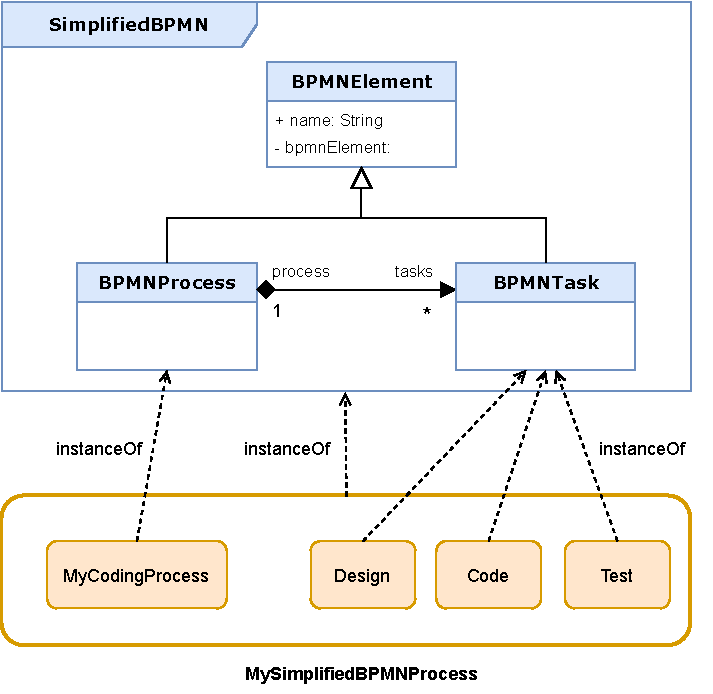
\includegraphics[width=\columnwidth]{Figures/BPMNSubsetExample.pdf}
    \caption{An example of BPMN subset built on top of a BPMN/EMF model}
    \label{fig:BPMNSubsetExample}
\end{figure}

\begin{lstlisting}
use org.openflexo.technologyadapter.emf.EMFModelSlot as EMF;
import ["http://www.omg.org/spec/BPMN/20100524/MODEL-XMI"] as BPMN_METAMODEL;

// A simplified BPMN metamodel exposing
// both concepts BPMNProcess and BPMNTask
model SimplifiedBPMN {

  // Connexion to a .bpmn file
  EMFModel bpmnModel 
    with EMF::EMFModelSlot(
        metaModel = BPMN_METAMODEL);

  // Abstract concept BPMNElement defining
  // a name and a link to an eventual BPMNElement
  // in .bpmn file
  abstract concept BPMNElement {
  	EMFObjectIndividual bpmnElement 
  	    with EMF::EMFObjectIndividualRole (
			source = bpmnModel
		);
    String name values bpmnElement.name;
  }

  concept BPMNProcess extends BPMNElement {

    // Describe here properties and
    // behaviours for BPMNProcess concept
    ...

    concept BPMNTask extends BPMNElement {

        // Describe here properties and
        // behaviours for BPMNTask concept
        ...

    }

    // Other core concepts
  }
}
\end{lstlisting}

\noteSylvain{Faut-il montrer des exemples de comportement aussi ?}


When the \FML execution engine runs a federation, it creates virtual
model instances containing concept instances. Some concept instances
are connected to external elements through model slot instances.


The tool support for model federation framework,
Openflexo\footnote{\url{https://github.com/openflexo-team}}, is
developed as an open source initiative. This tool offers a \FML
execution engine with an interactive virtual model design environment.

Finally, tools have their own model. We have taken advantage of
Openflexo features to build, in parallel with the models  required by the challenge, a drawing tool that makes our
solution (partially) executable.
